\section{Projeto da arquitetura}
A arquitetura proposta neste trabalho é baseada em camadas e utiliza os estilos arquiteturais \textit{Client-Server} e \textit{Event-Based}. O modelo em camadas possibilita manter a organização, a separação de conceitos e responsabilidades dos recursos da arquitetura, viabilizando a integração e comunicação entre os componentes através de conectores que podem ser definidos dinamicamente. No modelo em camadas, a conexão entre os componentes pode ser realizado tanto por eventos como por objetos compartilhados ou, através de leitura e escrita em um arquivo ou em uma base de dados. Porém, nesta arquitetura, foi utilizado somente eventos para comunicação entre os objetos da aplicação. A escolha de eventos como principal conector entre os objetos foi feita principalmente por proporcionar comunicação assíncrona entre emissor e ouvinte e pelo fato de não acoplar os componentes, garantindo maior independência entre os objetos e permitir que os plugins possam transmitir dados para outros objetos ou até mesmo outros plugins.\par


\subsection{Processos de desenvolvimento}
Esta arquitetura foi desenvolvida sob uma metodologia ágil com destaque para uma programação extrema e teste contínuo. A arquitetura recebeu alterações durante 10 meses e a primeira etapa de desenvolvimento introduziu o suporte aos plugins. O primeiro desafio foi desacoplar os plugins do arquivo QRC\footnote{QRC - Qt Resource Collection é um arquivo XML que mapeia os arquivos que serão empacotados no aplicativo} e permitir que a aplicação carregasse-os dinamicamente. Também nesta primeira etapa, foi implementado alguns recursos associados aos plugins, como controle de cache dos arquivos QML, ordenação e \textit{parsing} das páginas (definido pelos plugins), além da criação de um componente genérico a ser implementado por todas as páginas do aplicativo. O controle de cache consiste em regenerar o cache de todos os arquivos da aplicação após uma atualização e se faz necessário para garantir o carregamento de mudanças em cada arquivo a cada release. O componente genérico foi definido como \textit{BasePage.qml} e será detalhado posteriormente, ele foi criado para garantir o atendimento de alguns requisitos mínimos de aparência e estrutura da aplicação além de simplificar a criação de páginas. Na segunda etapa, foi implementado uma classe utilitária para que seus métodos fossem utilizados pelos plugins, oferecendo operações de baixo nível ainda não suportados pelo QML, pois nesta versão da arquitetura, ainda não é suportado a implementação de objetos c++ por conta dos plugins. Na terceira etapa, foi definido os layouts visuais suportados pela arquitetura e dois modelos foram implementados: O layout em pilha (faz uso do container \textit{StackView}) e o layout em linha (faz uso do container \textit{SwipeView}). O suporte ao layout deve ser definido no arquivo de configuração principal (à ser detalhado posteriormente), outros componentes serão instanciados para uso em conjunto com cada layout, dentre eles o TabBar e o ToolBar. Em etapas seguintes foi desenvolvido componentes visuais reutilizados na aplicação além das APIs para requisição HTTP e persistência de dados via QSLITE.


\subsection{Tecnologias utilizadas}
As tecnologias utilizadas consiste de todos os recursos que foram necessários para o desenvolvimento deste trabalho. O Qt e o \textit{QtCreator} foram os artefatos mais importantes, pois, forneceram os recursos e ferramentas para a construção das principais características da arquitetura. Dentre os recursos providos pelo Qt destaca-se os eventos, que permitem interligar objetos através de sinais e slots\footnote{funções javascript ou métodos de uma classe c++ invocados quando o sinal o qual estão conectados for emitido, recebendo em seus parâmetros os argumentos enviado pelo sinal.} ou \textit{signal handles}, e as APIs providas em classes C++ que integram os recursos da arquitetura, tais como, persistência de dados (via \textit{QSettings} e \textit{QSqlDatabase}) e rede (via \textit{QNetworkAccessManager}). O \textit{QtCreator} é uma IDE que possui recursos integrados à um projeto Qt e foi essencial para o desenvolvimento deste trabalho. Alguns recursos do \textit{QtCreator} destaca-se, facilidade de \textit{build} do projeto, construção do executável do aplicativo e o \textit{deploy} em um \textit{smartphone}, além de facilitar a realização de testes através de um mecanismo integrado de depuração. O \textit{QtCreator} também foi utilizado como editor de código fonte de todo o projeto da arquitetura.


% ver link: https://pt.slideshare.net/adrianotavares/modelagem-arquitetural-e-viso-41-presentation %
\subsection{Visão Geral da Arquitetura}
A visão a seguir, apresenta um diagrama de componentes da UML e exibe uma visão lógica dos principais pacotes e arquivos da arquitetura e logo a seguir, é descrito o papel e o conteúdo de cada um deles.

\begin{figure}[h]
	\includegraphics[scale=0.5]{diagrama_geral_da_arquitetura}
	\centering
	\caption{Pacotes principais da arquitetura}
\end{figure}

\begin{description}
	\item[1] \textit{tcc.pro}: Arquivo de configuração de todo projeto Qt. Nele é definido os módulos do Qt a serem utilizados na aplicação, as classes c++ que serão compiladas e linkadas no executável, os aquivos qrc que mapeiam os componentes QML, as imagens e arquivos genéricos a serem empacotados no executável, além de módulos e arquivos de configuração para cada plataforma (desktop, osx, android e ios). É neste arquivo que define onde os plugins serão instalados no dispositivo.

	\item[2] \textit{main.cpp}: Arquivo principal que define o ponto de entrada da aplicação. Responsável por instanciar as classes do Qt que exibem a janela do aplicativo e o interpretador de QML, além de classes da camada de aplicação, configuração e utilitários. O \textit{main} também é responsável por carregar os arquivos de tradução e registrar objetos no contexto da aplicação a serem utilizados pelos plugins.

	\item[3] \textit{config.json}: Arquivo de configuração principal desta arquitetura, pois define propriedades que indicarão alguns comportamentos iniciais e instância de objetos, tais como exibir os termos de uso na primeira inicialização do aplicativo (carregará o arquivo definido em \textit{assets/eula.html} definido pelo usuário da arquitetura), se tem login ou não, se usará layout em pilha e etc. Mais detalhes sobre esse arquivo será descrito em um tópico mais adiante.

	\item[4] \textit{src}: Diretório de código fonte. É onde está as classes c++ e componentes QML utilizados internamente e dispostos para plugins como componentes reusáveis. Esse diretório é sub-dividido em outros 5 diretórios que serão detalhados em outro diagrama.

	\item[5] \textit{plugins}: Diretório de plugins. Cada plugin deve obrigatóriamente estar em um sub-diretório com no mínimo um arquivo de configuração de nome \textit{config.json} e os arquivos QML e imagens que necessitar para o seu funcionamento. Os detalhes das propriedades requeridas para carregamento do plugin serão descritas em um tópico posterior.

	\item[6] \textit{translations}: Diretório contendo os arquivos de tradução. Os arquivos de tradução devem ser gerados ou atualizados antes de cada release do aplicativo. Um arquivo de resources \textit{translations.qrc} existe neste diretório e deve ser utilizado para mapear os arquivos de idioma suportados pelo aplicativo. Cada arquivo de tradução deve ser nomeado seguindo o padrão \textit{language\_COUNTRY} com extensão \textit{ts}, por exemplo: \textit{pt\_BR.ts}. Ao iniciar a aplicação, no arquivo \textit{main.cpp}, será identificado o \textit{locale} que define o idioma utilizado no dispositivo e o arquivo correspondente será instanciado para que as strings sejam exibidas traduzidas para o usuário. Para gerar as traduções, deve-se utilizar o comando \textit{lupdate tcc.pro} (na raíz do projeto) para criar ou atualizar o arquivo \textit{ts} principal.

	\item[7] \textit{android}: Diretório contendo os arquivos de configuração do aplicativo para a plataforma android. Outros sub-diretórios guardam arquivos do gradle utilizados para o build do APK, ícones do lançador do aplicativo e classes java, além de uma versão da lib \textit{openssl} compilada para o funcionamento de requisições HTTP.

	\item[8] \textit{assets}: Diretório contendo imagens e arquivos de configuração do \textit{qtquickcontrols2} além de um arquivo html que pode ser usado para exibir os termos de uso do aplicativo caso necessário. Um arquivo de \textit{resources} \textit{assets.qrc} mapeia todos os arquivos contidos neste diretório e pode ser usado para empacotar outros componentes e imagens do usuário no aplicativo.

	\item[9] \textit{ios}: Diretório contendo os arquivos de configuração do aplicativo para a plataforma ios. Pode conter os ícones do aplicativo além de imagens diversas requeridas pela plataforma tais como imagens de splash-screen, além do arquivo de configuração Info.plist.
\end{description}


\subsection{Arquitetura de plugins}
As funcionalidades de um aplicativo baseado nesta arquitetura deve ser implementado pelos plugins, seguindo as necessidades e os requisitos levantados para a aplicação a ser desenvolvida utilizando qml. Os plugins são independentes entre sí e podem incluir arquivos qml, txt, html e imagens em seu diretório. Qualquer componente de um plugin pode reutilizar os componentes públicos usando a diretiva \textit{import "qrc:/src/qml/"}. Os plugins estão desacoplados do núcleo da aplicação e serão conhecidos em tempo de execução. Ao adicionar um novo plugin no diretório \textit{plugins}, ele será carregado no próximo \textit{build} do projeto. Para que um plugin seja reconhecido pelo objeto gerenciador de plugins e carregado pela aplicação, é necessário obedecer a três restrições: estar em um sub-diretório dentro de \textit{plugins}, conter um arquivo \textit{config.json} e pelo menos um arquivo qml visual ou \textit{listener}. Os \textit{listeners} são componentes não visuais que observam eventos da aplicação. O arquivo \textit{config.json} deve ser um objeto contendo as seguintes propriedades:  
\begin{enumerate}
	\item \textit{name} (string): o nome do plugin (opcional);

	\item \textit{description} (string): uma descrição do plugin (opcional);

	\item \textit{pages} (array): uma lista de objetos que indentifica as páginas do plugin a serem exibidas no menu do aplicativo (requerido);

	\item \textit{listeners} (array): uma lista de strings que indentifica os arquivos do plugin (componentes qml não visuais) que serão instanciados como observadores de eventos (opcional).
\end{enumerate}

As páginas indicam objetos visuais que serão instanciadas sob demanda quando o aplicativo tiver utilizando o layout em pilha. No layout em pilha, um menu lateral estará disponível para que o usuário possa navegar nas páginas do aplicativo clicando em um item da lista.\par

Quando o layout em linha estiver sendo utilizado, uma lista horizontal de botões será posicionado no rodapé da janela do aplicativo permitindo ao usuário alternar entre as páginas disponíveis. Porém, no layout em linha, todas as páginas serão instanciadas no início da aplicação e terá um botão associado a cada página, adicionado em um objeto \textit{TabBar}. Cada objeto em \textit{pages} poderá conter as seguintes propriedades que serão lidas pelos componentes que definem os menus durante a inicialização do aplicativo:

\begin{itemize}
	\item \textit{qml} (string): O nome do arquivo correspondente a página. Se esse valor não for definido, a página não será carregada.

	\item \textit{title} (string): O título correspondente a página a ser exibido no menu. Esse valor também é requerido, se não for definido, a página não será carregada.

	\item \textit{icon} (string) (requerido): O nome de um ícone do \textit{Awesome Icons} que será exibido no menu, em conjunto com o título. Se esse valor não for definido, um ícone padrão será utilizado.

	\item \textit{roles} (array): Uma lista de strings contendo os nomes de perfil de usuário que poderão acessar a página. Esse array será útil somente se a aplicação definir o tipo de perfil do usuário no objeto \textit{UserProfile.profile}. Esse valor é opcional, caso não for definido, será setado um array vazio. Porém, se for definido o perfil do usuário no objeto \textit{profile} e essa string não tiver nesta propriedade (\textit{roles}), a página não será exibida.

	\item \textit{order} (integer): Um valor numérico que define a ordem em que a página será exibida na lista de itens nos menus. O desenvolvedor deverá definir um valor acima de zero e quanto maior o valor, maior a prioridade na lista de itens.

	\item \textit{isLoginPage} (boolean): Um flag que indica se a página é o login e deve ser definido se o valor da propriedade \textit{usesLogin} for definido para true no \textit{config.json} do projeto. Se o aplicativo usa login, o \textit{path} da página definida como login será persistido para seja carregado por funções internas do aplicativo na inicialização e quando o usuário fizer \textit{logout}.

	\item \textit{isHomePage} (boolean): Um flag que indica se a página corresponde a primeira página exibida para o usuário. Se for definido para \textit{true}, o \textit{path} desta página será persisitido e será carregada após o login. No entanto, se o aplicativo não usa login, o aplicativo carregará a página definida como \textit{homePage} na inicialização e será a primeira página exibida para o usuário. Essa propriedade é opcional e deve ser definida somente pela página correspondente.

	\item \textit{showInDrawer} (boolean): Um flag que indica se a página poderá ser exibida no menu de layout em pilha, que neste caso é uma instância do objeto \textit{Drawer}. O menu \textit{Drawer} pode ser instanciado mesmo no layout em linha, basta definir a propriedade \textit{usesDrawer} para \textit{true} no arquivo de configuração. Neste caso, o layout em linha utiliza o \textit{TabBar} como menu e dessa forma será possível exibir páginas diferentes nos dois menus.

	\item \textit{showInTabBar} (boolean): Um flag que indica se a página poderá ser exibida no menu de layout em linha, que corresponde ao \textit{TabBar}, posicionado no rodapé da janela do aplicativo. O objetivo desse flag é permitir exibir páginas diferentes nos menus quando o \textit{Drawer} menu estiver sendo utilizado.
\end{itemize}

No layout em pilha, o menu é exibido pelo componente \textit{Menu.qml} que consiste de uma instância do objeto \textit{Drawer} do \textit{QuickControls} e as páginas serão listadas verticalmente. No layout em linha, o menu corresponde ao componente \textit{TabBar.qml} também do \textit{QuickControls} com algumas modificações. É importante destacar que os plugins serão carregados e persistidos na primeira inicialização em um array de objetos. No entanto, esse array será reconstruído quando a aplicação estiver sendo executada em modo \textit{debug} ou desktop, para que novos plugins sejam carregadas sem necessitar a limpeza do cache do aplicativo durante o desenvolvimento. Em modo \textit{release}, por questões de desempenho, o aplicativo carregará as plugins a partir da persistência local do aplicativo. Os plugins serão lidos a cada release após atualização da versão do aplicativo.\par


%adicionar um diagrama de componentes mostrando os plugins em um diretório de plugins e outros diretórios da aplicação
\subsubsection{Gerenciamento de plugins}\label{sec:solucao-desenvolvida}
A classe \textit{PluginManager} é responsável por carregar os plugins, ela é instanciada no objeto \textit{App} na inicialização do aplicativo. Basicamente, o que esta classe faz é iterar todos os arquivos dentro do diretório \textit{plugins} e analizar as propriedades definida no arquivo \textit{config.json} de cada plugin. Em cada arquivo, é verificado as propriedades definida para cada página adicionando-a como objeto em um array. Após ler todos os plugins, o array de objetos é persistido nas configurações da aplicação para que na próxima inicialização não precise iterar novamente o diretório, lendo as definições dos plugins das configurações, exceto se houver uma atualização da aplicação ou quando a aplicação é executada em modo \textit{debug}. A cada inicialização, é feito uma verificação da versão do aplicativo, que também é persistido nas configurações, se houver alguma diferença entre versão em execução da versão salva se existir, os plugins serão recarregados. Além disso, esta classe também é reponsável por deletar todos os arquivos de cache contido no diretório de cache da aplicação a cada release. Outra responsabilidade dessa classe, é a criação da tabela do plugin em banco de dados \textit{SQLITE} se o plugin fornecer um arquivo \textit{plugin\_table.sql} em seu diretório. O banco de dados da aplicação é criado por um objeto que gerencia as operações de presistência e será detalhado em outro tópico. O diagrama a seguir, apresenta detalhes da classe \textit{PluginManager}.

\begin{figure}[h]
	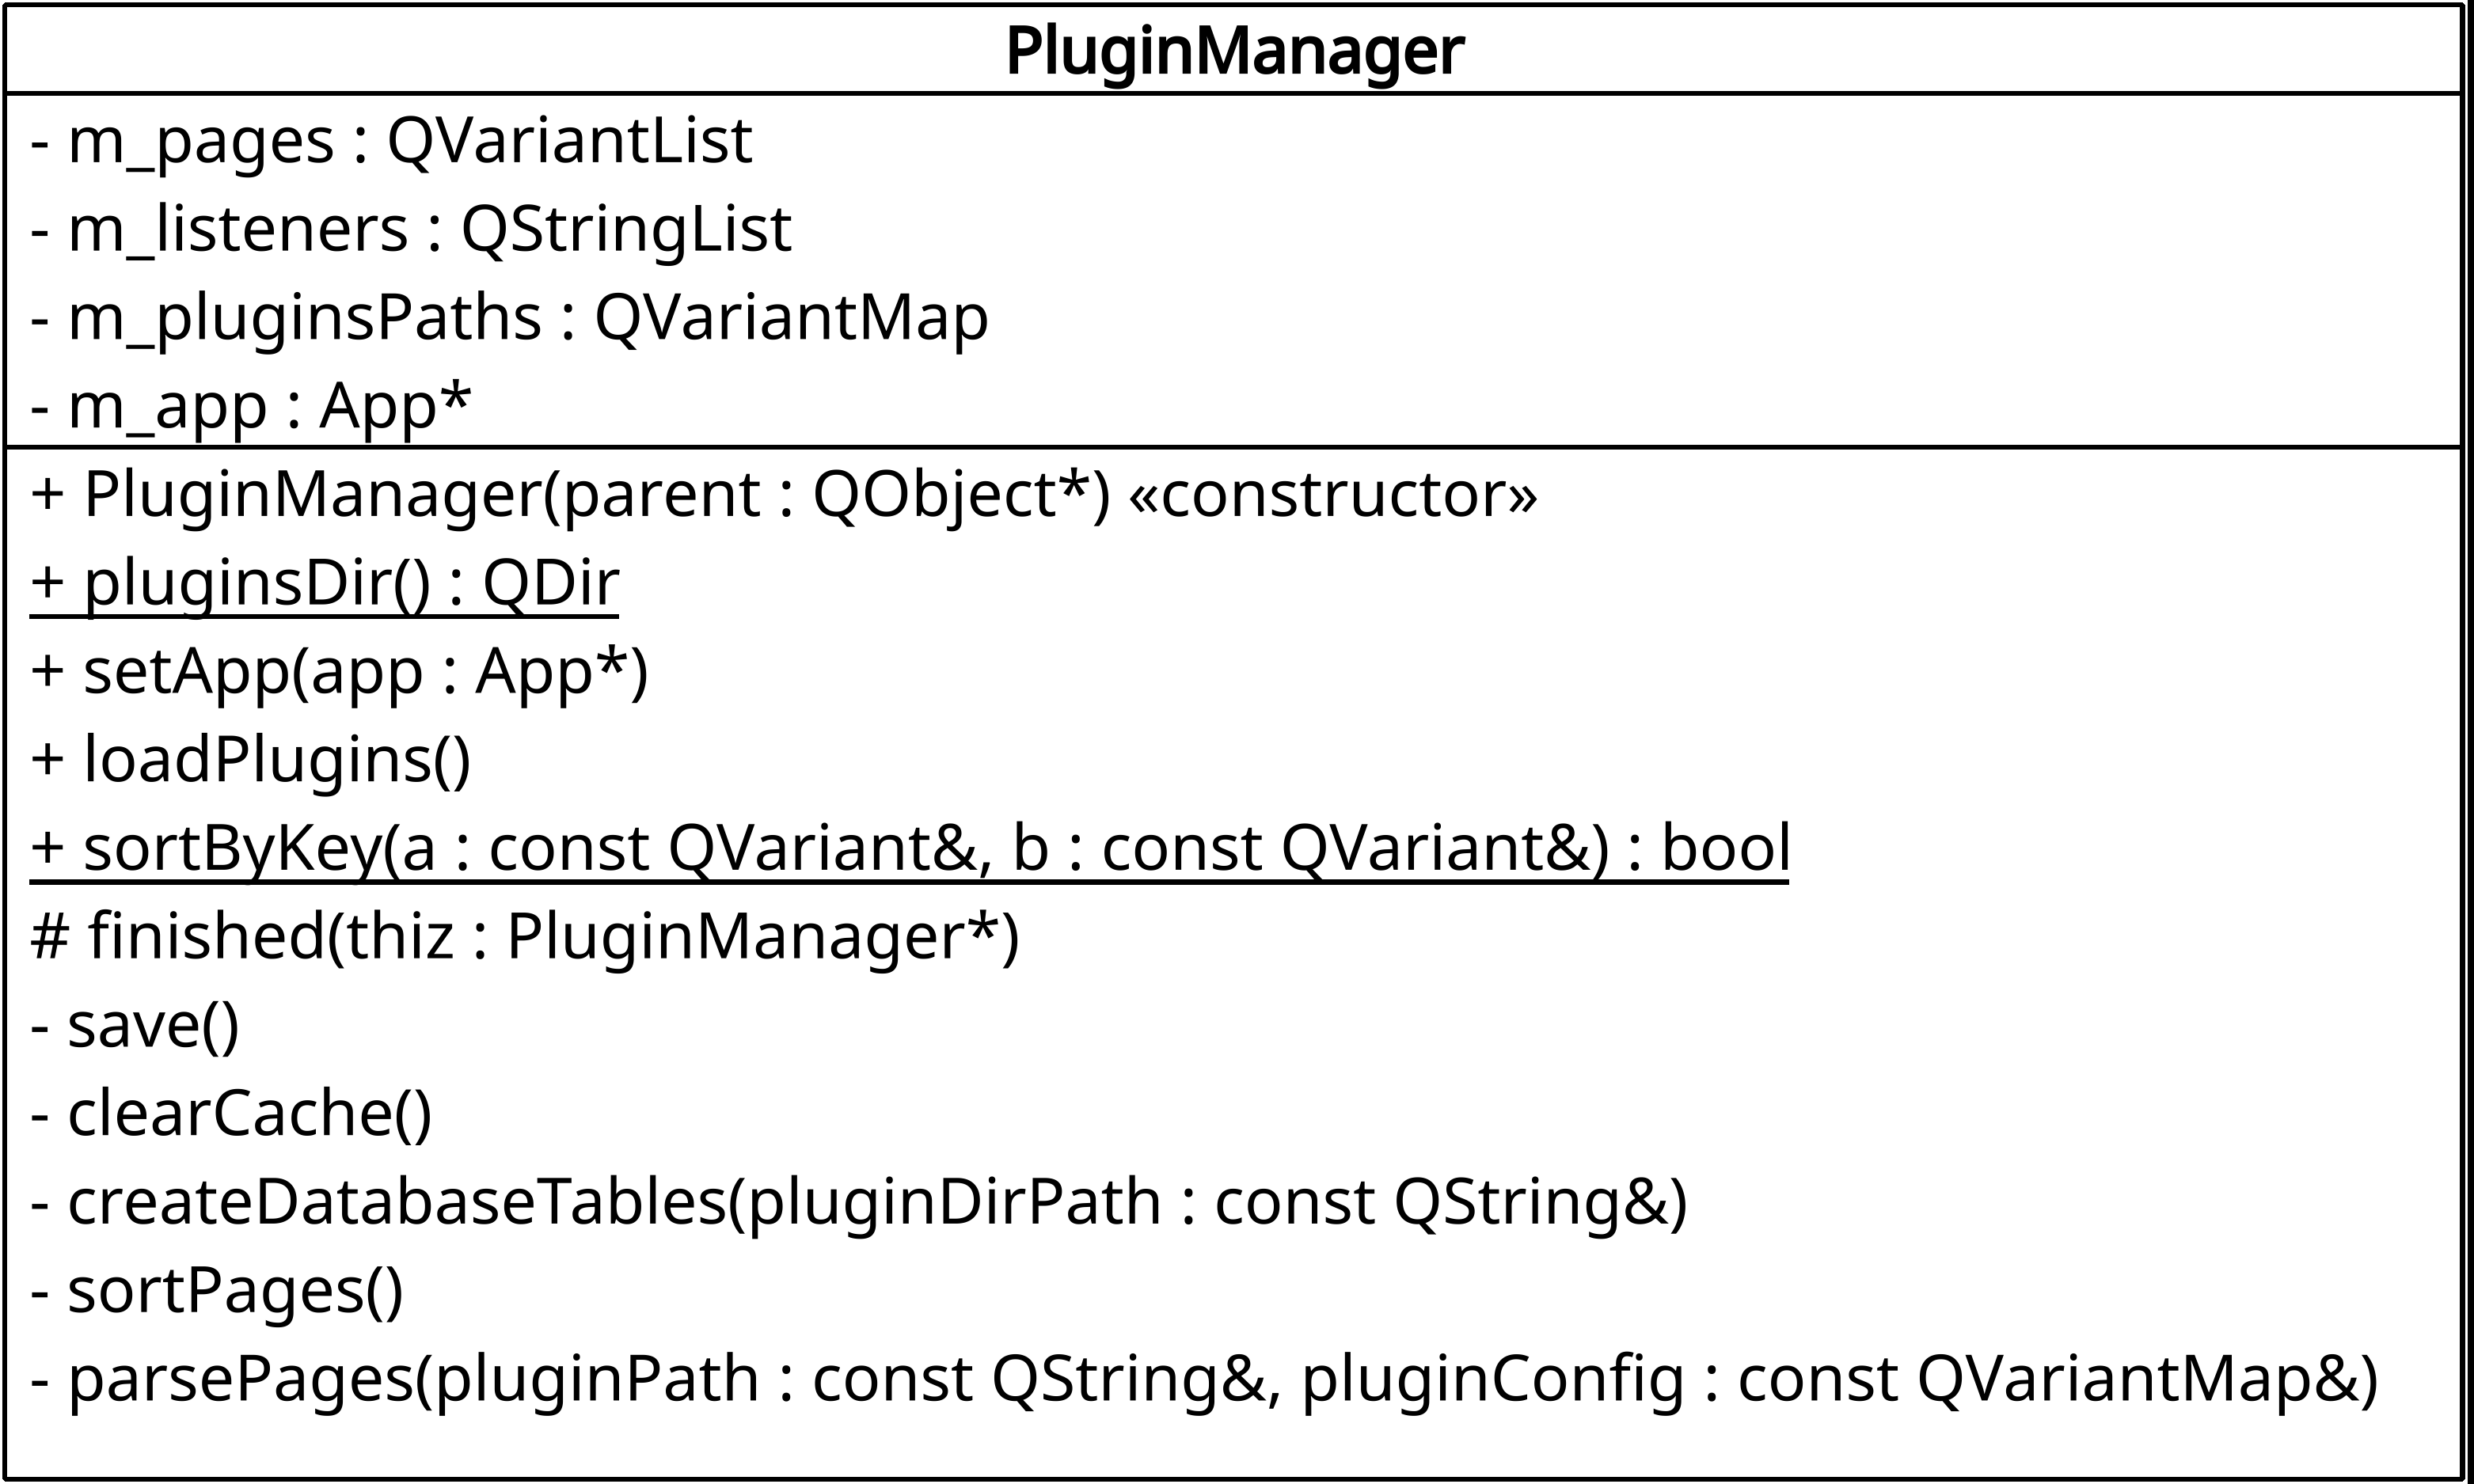
\includegraphics[width=8cm]{diagrama_de_classe_PluginManager}
	\centering
	\caption{Diagrama da classe PluginManager}
\end{figure}

\subsection{O arquivo config.json}\label{sec:solucao-desenvolvida}
O arquivo \textit{Settings.json} é um arquivo importante e requerido nesta arquitetura. As propriedades presentes neste arquivo não são persistidas no banco de dados e serão setadas em um objeto do tipo \textit{QVariantMap} na classe App, sempre que o aplicativo for executado. Este objeto será registrado no contexto da aplicação como uma propriedade e será utilizado por vários componentes, tais como, elementos visuais que definem cores, font-size e outras propriedades que podem ser definidas neste json e poderão ser acessadas por qualquer plugin. Algumas propriedades como versão do aplicativo e se está ou não em modo de depuração. O número da versão é especificado na chave \textit{version} e é utilizado pelo objeto ManagerPlugins que decidirá se o cache dos arquivos QML serão deletados para que os arquivos QML presentes na nova versão sejam regenerados. será utilizado por mapear tanto o tema de cores utilizado pelos componentes visuais como também detalhes de nome, versão e descrição do aplicativo.


%adicionar um diagrama de componentes mostrando os plugins em um diretório de plugins e outros diretórios da aplicação
\subsection{O Qt e o QML}\label{sec:solucao-desenvolvida}
Para compreender a implementação deste trabalho é importante entender os recursos do Qt e como ele facilitou o desenvolvimento desta arquitetura. O Qt é a base da implementação deste trabalho, ele provê um conjunto de bibliotecas, classes e componentes além de uma infraestrutura de desenvolvimento, depuração e deploy. O Qt também fornece APIs de alto nível que abstrai a plataforma e o sistema operacional e permite integrar objetos através de um mecanismo de comunicação orientado a eventos. O Qt consiste de um kit de ferramentas composto de classes C++, um interpretador de linguagem declarativa chamada QML além de Módulos com APIs de rede, persistência de dados, recursos de hardware como câmera, bluetooth, sensores e etc. Além de uma ampla de componentes visuais de alto nível que facilitam a construção de interface gráfica. Os elementos seguintes são áreas-chave de funcionalidades do Qt \cite{qt_overviews}.

\begin{itemize}
	\item Ferramentas de Desenvolvimento através da IDE Qt Creator que fornece depuração e deploy simplificado
	\item Armazenamento de dados em alto nível de abstração e independente de plataforma
	\item Suporte a rede (http) e conectividade também independente de plataforma
	\item Gráficos proeminentes providos pelo QML através do módulo \textit{Qt Quick} e \textit{Quick Controls}
	\item Portabilidade com alta abstração de plataforma para elementos visuais como imagens, botões e exibição de textos
	\item Desenvolvimento aberto através da licença open source
\end{itemize}

\subsection{Comunicação entre os componentes}
Esta seção descreve o processo de comunicação entre objetos ou componentes dentro do aplicativo...


\section{Aspectos de Implementação}\label{sec:solucao-desenvolvida}
Nesta sessão é discutido detalhes da solução desenvolvida. Será apresentado nas subseções seguintes os componentes que integra a arquitetura desenvolvida, descrevendo as decisões e características de implementação de cada componente.


\subsection{O Objeto App}\label{sec:solucao-desenvolvida}
O objeto app é um componente importante nesta arquitetura, ele gerencia toda a persistência de dados através de uma instância da classe \textit{QSettings} que abstrai a plataforma e fornece um mecanismo para leitura e escrita de dados no dispositivo através de métodos parametrizados. O objeto app é também o responsável por instanciar a classe \textit{PluginManager}, que realiza o trabalho de carregar os plugins do aplicativo. Outra responsabilidade deste objeto, é a notificação de eventos vindos do objeto \textit{QtActivity} no android e \textit{QtAppDelegate} no iOS como o \textit{token} de registro no \textit{Firebase}\footnote{O Firebase antigo \textit{Google Cloud Messaging} é um serviço de notificação móvel desenvolvido pelo Google que permite que os desenvolvedores de aplicativos enviem dados ou informações de notificação de servidores executados pelo desenvolvedor para aplicativos Android e iOS.} e mensagens de \textit{push notification} que em ambos os eventos, são delegados para o aplicativo através de uma conexão com um \textit{slot} definido no \textit{Application Window}.

\begin{figure}[h]
	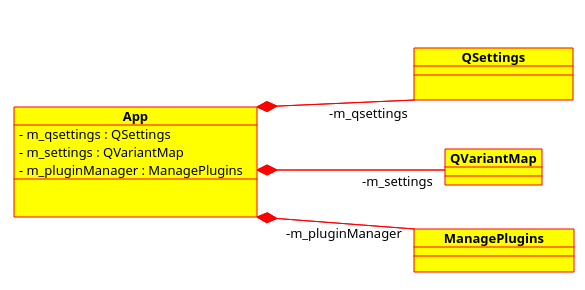
\includegraphics[width=8cm]{a_classe_app}
	\centering
	\caption{Os objetos compostos da classe App}
\end{figure}

O Objeto App também fornece métodos públicos declarados como 


\subsection{Gerencimento de Rede (HTTP)}\label{sec:solucao-desenvolvida}
\subsubsection{O Componente RequestHttp}\label{sec:solucao-desenvolvida}
O Objeto RequestHttp....


\subsection{Gerencimento de Banco de Dados}\label{sec:solucao-desenvolvida}
\subsubsection{O Componente Database}\label{sec:solucao-desenvolvida}
O Objeto ModelData....


\subsection{O Componente Basepage}\label{sec:solucao-desenvolvida}
O Objeto ModelData....


\subsection{Componentes Visuais}\label{sec:solucao-desenvolvida}
O Objeto ModelData....



\subsection{Métodos para utilização da arquitetura}
-- descrever o README do projeto no github

OU:
Exemplo (a ser editado): Para se utilizar a arquitetura desenvolvida, deve-se seguir uma determinada ordem de atividades (Figura 26), que deve se iniciar no nível arquitetural “escopo” (seção 3.1), passando pelos níveis arquiteturais “modelo de negócios” (seção 3.2) e “modelo de sistema” (seção 3.3), até chegar ao nível arquitetural “modelo tecnológico” que deve ser criado pelo usuário desta arquitetura.